\begin{comment}
\begin{gnuplot}[terminal=epslatex, terminaloptions=color dashed, terminaloptions={size 8cm,5cm}]
a(x) = x>0 ? 1 : -1
set samples 10000
set key at -1.4,1.25

set xrange[-5.0:5.0]
set yrange[-1.5:1.5]

set format x "\%1.1f"
set format y "\%1.1f"

plot a(x) lc rgb "red" lw 4
\end{gnuplot}
\end{comment}

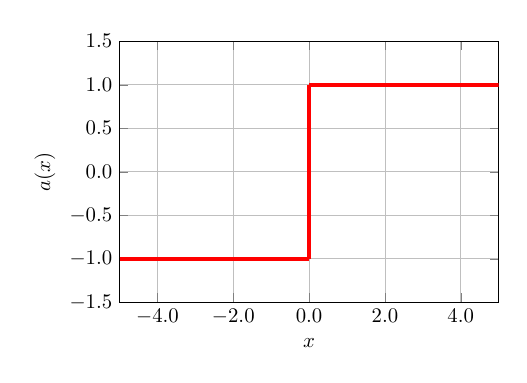
\begin{tikzpicture}[scale=0.75]
\begin{axis}[
width=8cm, height=6cm,
xmin=-5, xmax=5,
ymin=-1.5, ymax=1.5, 
grid, 
xlabel=$x$, ylabel=$a(x)$,
xtick = {-4.0,-2.0,0,2.0,4.0},
ytick = {-1.5,-1.0,-0.5,0,0.5,1.0,1.5},
y tick label style={/pgf/number format/.cd,%
        fixed,
        fixed zerofill,
        precision=1},
x tick label style={/pgf/number format/.cd,%
        fixed,
        fixed zerofill,
        precision=1}
]

\draw[line width=2.pt,color=red] (-5,-1) -- (0,-1);
\draw[line width=2.pt,color=red] (0,-1) -- (0,1);
\draw[line width=2.pt,color=red] (0,1) -- (5,1);

% \addplot[red,smooth] gnuplot[id=step]{x>0 ? 1 : -1};

% \addplot[red,smooth] {tanh(x)};

\end{axis}
\end{tikzpicture}